\documentclass[11pt]{article}
\usepackage{learn}
\usepackage{tikz}
\title{Semaphores: Counting Permits}
\author{}
\date{}
\begin{document}
\maketitle

\section{The answer in two sentences}
A \textbf{semaphore} is an integer counter plus two atomic operations: \code{wait} (also called $P$ or acquire) decrements it and blocks if it would go negative, and \code{signal} (also $V$ or release) increments it and wakes a blocked waiter. It is a mutex generalized from ``one holder at a time'' to ``$N$ holders at a time.''

\section{Plain definition}
A semaphore is a concurrency primitive that controls how many threads may pass a checkpoint simultaneously. You initialize it with a count $N$; each thread that wants in calls \code{wait}, and each thread that leaves calls \code{signal}. In your problem, if you have a pool of 4 database connections and 20 worker threads, the semaphore is the bouncer that lets exactly 4 through and parks the other 16.

\section{Intuition from first principles}
You already know a mutex: a lock with count 1. It answers ``may I enter?'' with yes or no. But some resources are not single: a buffer with 8 free slots, a thread pool with 4 workers, a printer with 2 trays. You want the same mutual-exclusion machinery, but with a budget. The natural object is a counter: start at $N$, decrement on entry, increment on exit, block when the decrement would take you below zero. That is the whole idea. The only subtlety is that the decrement-and-check must be atomic, otherwise two threads can both see ``1 left'' and both enter.

\section{Mechanism}
The counter lives in kernel (or runtime) memory, guarded by a short internal lock. \code{wait} does: lock, if count $> 0$ then count $-=$ 1 and return, else enqueue the calling thread and sleep; unlock. \code{signal} does: lock, if a waiter is queued, wake one, else count $+=$ 1; unlock. \underneath{The internal lock is held only for a few instructions; the sleeping happens outside it.}

\begin{center}
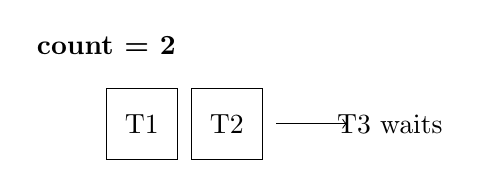
\begin{tikzpicture}[scale=0.9]
\node at (0,1.6) {\textbf{count = 2}};
\draw (0,0) rectangle (1,1); \draw (1.2,0) rectangle (2.2,1);
\node at (0.5,0.5) {T1}; \node at (1.7,0.5) {T2};
\node at (4,0.5) {T3 waits};
\draw[->] (2.4,0.5) -- (3.4,0.5);
\end{tikzpicture}
\end{center}

Two threads hold permits; a third blocks in \code{wait} until one calls \code{signal}. There are two flavors: a \textbf{counting semaphore} (any $N \ge 0$) and a \textbf{binary semaphore} ($N \in \{0,1\}$, which is a mutex with different ownership rules). A mutex is owned by the thread that locked it; a semaphore is not, so any thread may \code{signal}. That is a feature (producer/consumer handoff) and a footgun (you can signal too many times).

\section{Worked example}
A bounded buffer: producers append, consumers remove, capacity 3. A counting semaphore tracks free slots; another tracks filled slots.

\begin{lstlisting}[style=py]
import threading
free_slots = threading.Semaphore(3)
filled     = threading.Semaphore(0)

def producer(item):
    free_slots.acquire()   # wait: block if buffer full
    buf.append(item)
    filled.release()       # signal: one more item

def consumer():
    filled.acquire()       # wait: block if empty
    item = buf.pop(0)
    free_slots.release()   # signal: one more slot
    return item
\end{lstlisting}

Trace: start with \code{free\_slots=3, filled=0}. Three producers run, buffer is full, \code{free\_slots=0}. A fourth producer calls \code{acquire} and blocks. A consumer calls \code{filled.acquire} (count 1, passes), pops, then \code{free\_slots.release} wakes the blocked producer. Note the two semaphores are mirror images: one counts emptiness, one counts fullness.

\section{Common pitfalls}
\begin{itemize}[leftmargin=1.2em]
\item \textbf{Forgetting to release on the error path.} If an exception skips \code{release}, the permit leaks and the pool shrinks forever. Use \code{with sem:} in Python or a RAII guard in C++.
\item \textbf{Signaling before waiting.} A semaphore is not a queue of messages; if you \code{release} more times than \code{acquire}, the count grows and the gate stays open. Match every wait with exactly one signal.
\item \textbf{Using a semaphore where a mutex belongs.} For pure mutual exclusion, a mutex is clearer and enforces ownership. Reach for a semaphore only when the count is genuinely $>1$.
\item \textbf{Assuming fairness.} Most implementations do not guarantee FIFO wakeup; a thread can starve. If order matters, use a condition variable with an explicit queue.
\end{itemize}

\begin{keypoint}[title={Reference}]
\textbf{State:} integer count $\ge 0$ (plus a waiter queue).\\
\textbf{wait / P / acquire:} count $-=$ 1; block if it would go negative.\\
\textbf{signal / V / release:} count $+=$ 1; wake one waiter if any.\\
\textbf{Binary semaphore} = mutex without ownership. \textbf{Counting} = budget of $N$.\\
\textbf{Invariant:} count + (threads inside) = initial $N$.\\
\textbf{Cost:} uncontended wait/signal is a few atomic instructions; contended blocks the thread.\\
\textbf{Python:} \code{threading.Semaphore(n)}, \code{acquire()}, \code{release()}, supports \code{with}.\\
\textbf{C++:} \code{std::counting\_semaphore} (C++20), \code{acquire()}, \code{release()}.
\end{keypoint}

\section{Check yourself}
\begin{enumerate}[leftmargin=1.2em]
\item A semaphore starts at 5. Ten threads call \code{wait}, then three call \code{signal}. What is the count and how many threads are blocked?
\item Why must the decrement-and-check in \code{wait} be atomic?
\item You have a mutex and a binary semaphore. Name one behavior that differs.
\end{enumerate}

\subsection*{Answers}
\small
1. Count is 3; seven threads are blocked (five passed, three of the ten were released). 2. Otherwise two threads can both observe count $=1$ and both enter, exceeding the budget. 3. Ownership: only the locking thread may unlock a mutex; any thread may signal a semaphore.

\section{Go further}
Python docs on \code{threading.Semaphore}: \url{https://docs.python.org/3/library/threading.html\#semaphore-objects}. Next, learn \textbf{condition variables}: a semaphore is essentially a counter plus a condition variable, and understanding the underlying wait/notify lets you build your own.

Stuck on any part? Press c and ask.
\end{document}
